%%%%%%%%%%%%%%%%%%%%%%%%%%%%%%%%%%%%%%%%%%%%%%%%%%%%%%%%%%%%%%%%%%%%%%%%%%%%%%%%
%2345678901234567890123456789012345678901234567890123456789012345678901234567890
%        1         2         3         4         5         6         7         8


\documentclass[letterpaper, 10 pt, conference]{ieeeconf}  % Comment this line out if you need a4paper

%\documentclass[a4paper, 10pt, conference]{ieeeconf}      % Use this line for a4 paper

\IEEEoverridecommandlockouts                              % This command is only needed if 
                                                          % you want to use the \thanks command

\overrideIEEEmargins                                      % Needed to meet printer requirements.

%In case you encounter the following error:
%Error 1010 The PDF file may be corrupt (unable to open PDF file) OR
%Error 1000 An error occurred while parsing a contents stream. Unable to analyze the PDF file.
%This is a known problem with pdfLaTeX conversion filter. The file cannot be opened with acrobat reader
%Please use one of the alternatives below to circumvent this error by uncommenting one or the other
%\pdfobjcompresslevel=0
%\pdfminorversion=4

% See the \addtolength command later in the file to balance the column lengths
% on the last page of the document

% The following packages can be found on http:\\www.ctan.org
%\usepackage{graphics} % for pdf, bitmapped graphics files
%\usepackage{epsfig} % for postscript graphics files
%\usepackage{mathptmx} % assumes new font selection scheme installed
%\usepackage{times} % assumes new font selection scheme installed
%\usepackage{amsmath} % assumes amsmath package installed
%\usepackage{amssymb}  % assumes amsmath package installed
\usepackage{graphicx}
\usepackage{amsmath,amsfonts}
\usepackage{multirow} 
\usepackage{amssymb}
\usepackage{array}
\usepackage{booktabs}
\usepackage{caption}


\title{\LARGE \bf
CedarSAM: Fine-Tuning Segment Anything Model for Semantic Segmentation of Eastern Red Cedar Vegetation from UAV Imagery
}

\author{Minji Lee$^{1}$ and Eric T. Matson$^{2}$% <-this % stops a space
%\thanks{*This work was supported by Purdue University}% <-this % stops a space
\thanks{$^{1}$Minji Lee is a Ph.D., Candidate, Computer and Information Technology, Purdue University, West Lafayette, IN, 47906, USA
        {\tt\small lee3450@purdue.edu}}%
\thanks{$^{2}$Eric T. Matson is a Professor in Computer and Information Technology, West Lafayette, IN, 47906, USA
        {\tt\small ematson@purdue.edu}}%
}


\begin{document}



\maketitle
\thispagestyle{empty}
\pagestyle{empty}


\begin{abstract}
Although the Segment Anything Model has demonstrated remarkable generalization ability in zero-shot segmentation tasks, its performance on specialized or domain-specific imagery, such as aerial vegetation images, may fall short of the precision required for real-world applications. This study investigates the effectiveness of fine-tuning CedarSAM on a small and labeled dataset of aerial tree images to enhance segmentation performance for a specific tree species — Eastern Red Cedar. Despite the limited dataset size, the results show that the CedarSAM model achieves notable improvements in segmentation accuracy across multiple metrics, including Dice score, Intersection over Union, Precision, Recall, and Inference time. These findings highlight the potential of domain adaptation with minimal data, enabling practitioners to deploy SAM effectively in niche applications without the need for large-scale datasets.
\end{abstract}

\section{INTRODUCTION}
The Segment Anything Model (SAM), developed by Meta AI [1], provides several demos showcasing its zero-shot segmentation capabilities across a wide range of objects and scenes, in its dataset, available at the Segment Anything Dataset (SA-1B). Developed as a foundational model for segmentation tasks, SAM leverages a transformer-based architecture trained on millions of images to provide powerful prompt-based segmentation capabilities. However, when applied to specialized domains with unique visual characteristics such as medical imaging, or ecological monitoring, the model's performance may not always achieve optimal results [2][3]. In particular, SAM’s performance significantly decreases when multiple objects overlap or exhibit irregular shapes, which is common in natural environments [4][5].

\begin{figure}[thpb]
  \centering
  \framebox{\parbox{3in}{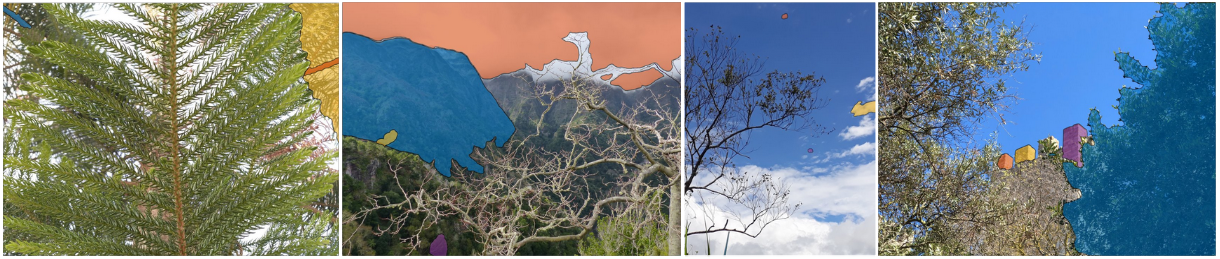
\includegraphics[width=\linewidth]{sam_figures.png}}}
  \caption{Challenges of SAM in vegetation segmentation: Under-segmentation in complex natural environments.}
  \label{fig:score_distributions}
\end{figure}

Figure 1 illustrates the challenges faced by SAM when applied to complex vegetation scenes. Despite its generalization ability, SAM demonstrates under-segmentation in densely foliated environments with overlapping elements and intricate textures. For instance, in the image with the ID sa-1854685 (first from the left), the model detected only three masks in total even though numerous leaves are visible. Similarly, images with IDs sa-2087535 (second from the left), sa-3186430 (third from the left), and sa-8315875 (rightmost) exhibit under-segmentation, with only four masks detected in each case. These examples highlight SAM's limitations in identifying detailed structures in vegetation-rich scenes, emphasizing the need for domain-specific fine-tuning to improve segmentation accuracy.

The Eastern Red Cedar (ERC) tree was selected as the target object for this study due to its ecological dominance and rapid spread in agricultural environments. As an invasive species in certain regions [6], it has the potential to outcompete native vegetation and reduce biodiversity. Monitoring and managing the spread of ERC is therefore critical for ecological conservation efforts [7][8]. To accurately capture its presence and distribution, aerial imagery was collected using an UAV equipped with a high resolution camera (6K). UAVs offer an efficient and cost-effective solution to obtain datasets in forested and rural areas, providing detailed visual data compared to other remote sensing methods [9][10]. Unlike radar, which uses radio waves to detect objects and is typically used for large-scale geological mapping or weather monitoring, UAV imagery provides high resolution visual information that captures detailed surface features. Similarly, while LiDAR (Light Detection and Ranging) uses laser pulses to create precise 3D models of terrain and vegetation, it often requires specialized sensors and can be costly [11].

This study investigates the effectiveness of fine-tuning SAM using a small labeled aerial image dataset to improve segmentation performance of ERC and evaluates its efficiency for ecological monitoring applications. The primary research questions that guide this study are (1) How effectively can SAM be fine-tuned with a small domain-specific dataset? (2) What performance improvements can be expected on various evaluation metrics? (3) What are the trade-offs between model performance and computational efficiency after fine-tuning?

This research also includes a comparative analysis between the original SAM and a fine-tuned variant, CedarSAM, across multiple evaluation criteria, including dice coefficient, Intersection over Union (IoU), precision, recall, and inference time. The results demonstrate that even with limited training data, targeted fine-tuning can yield improvements in segmentation quality while maintaining computational efficiency. These findings allow for the adaptation of foundation models to specific domains without the need for extensive data collection.

\begin{figure*}[thpb]
  \centering
  \framebox{\parbox{\textwidth}{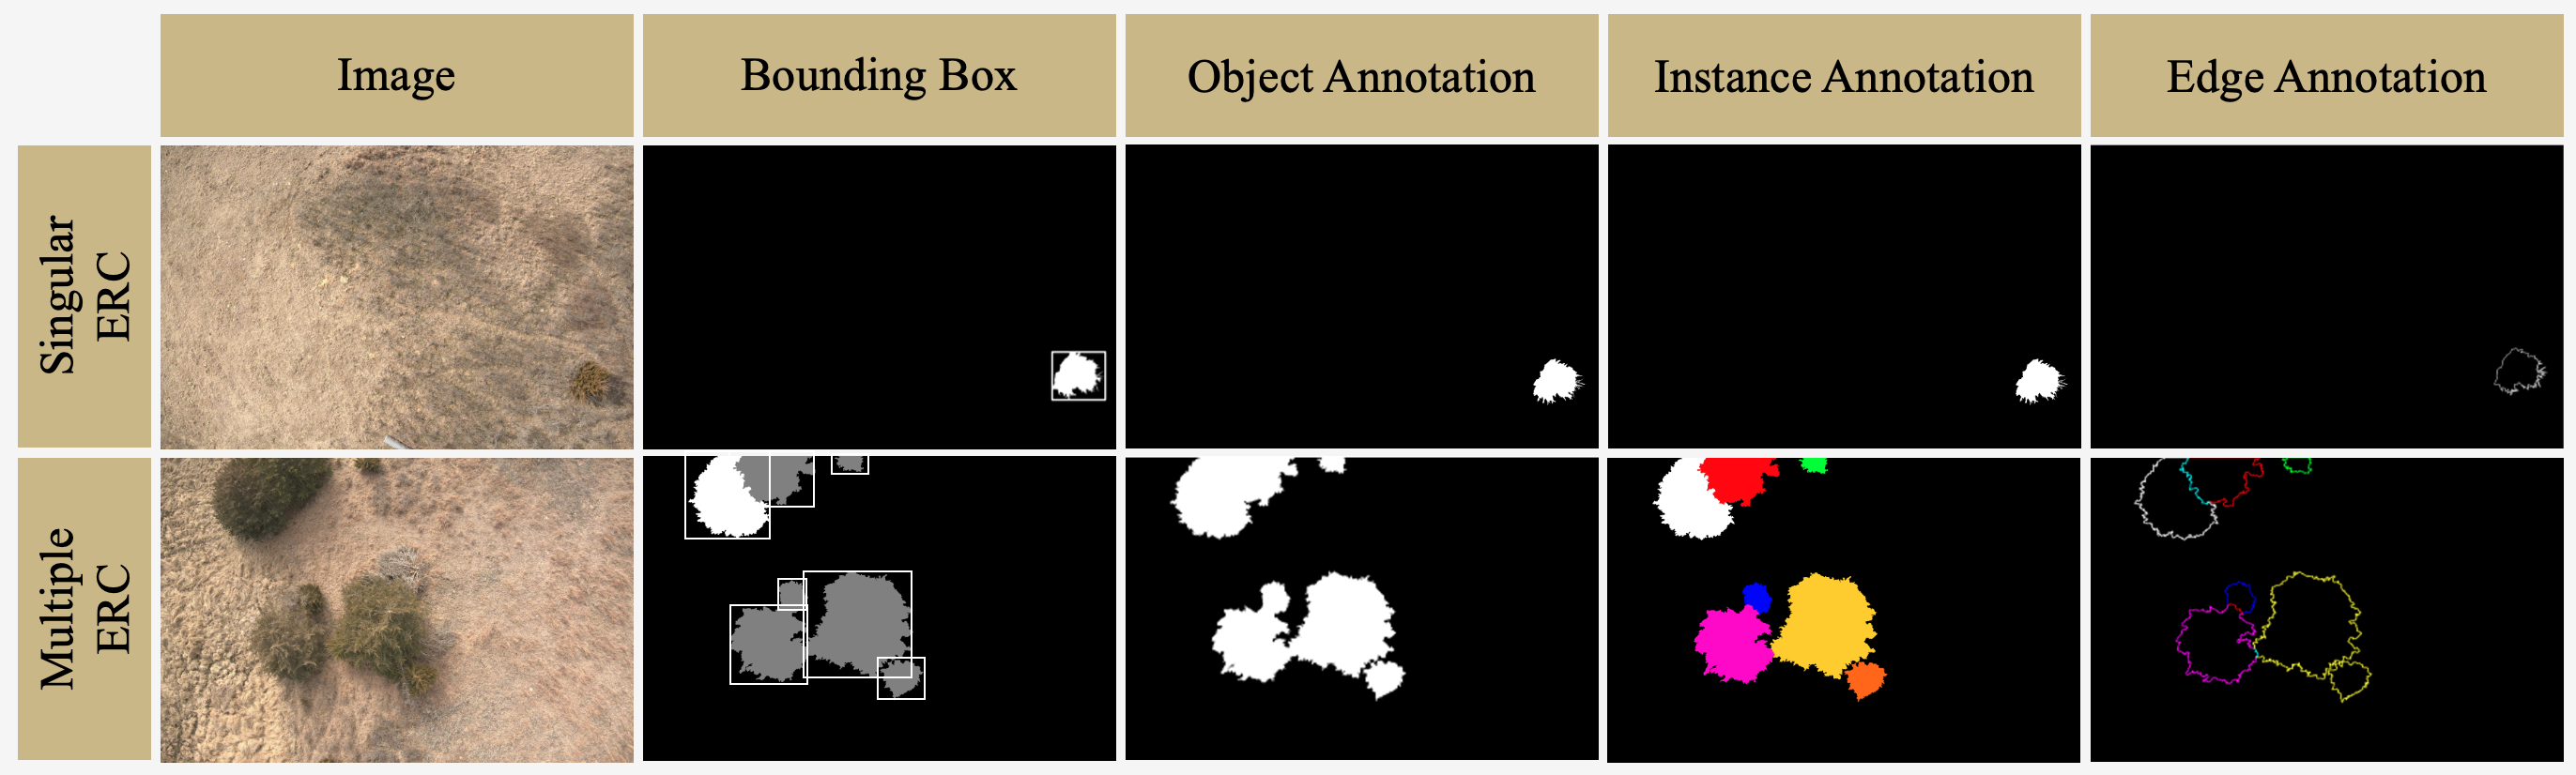
\includegraphics[width=\textwidth]{sam_images.png}}}
  \caption{Annotation diversity in the proposed CedarSAM dataset. Unlike previous works that only provide coarse-grained object-level annotations, this dataset offers four different annotation types for each image: bounding boxes (2nd column), object annotations (3rd column), instance annotations (4th column), and edge annotations (5th column). These diverse annotations support various prompt types, such as masks or boxes, for the SAM model.}
  \label{fig:score_distributions}
\end{figure*}

\section{Methodology}

\subsection{Dataset Preparation}
The dataset consists of 106 high resolution images (5472 × 3648), including 85 images for training and 21 for validation. The images were acquired using an Autel Robotics EVO II XT705 drone, representing typical ecological monitoring scenarios where vegetation assessment is critical. The images contain diverse vegetation patterns, including isolated shrubs, clustered vegetation patches, and mixed vegetation at different growth stages from a range pasture in western Kansas. This diversity presents significant segmentation challenges due to variations in vegetation density, color, and texture against the soil background, as shown in Figure 3.

\begin{figure}[thpb]
  \centering
  \framebox{\parbox{3in}{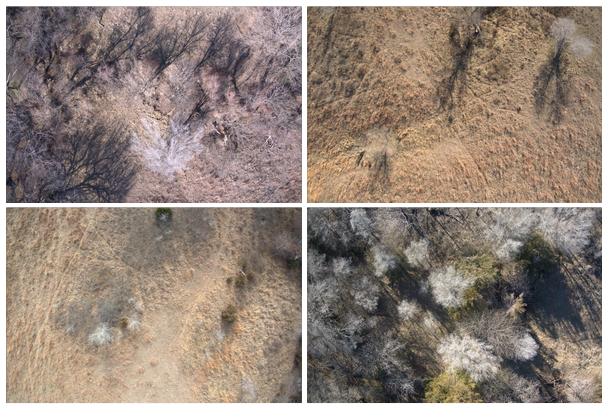
\includegraphics[width=\linewidth]{sam_examples.png}}}
  \caption{Diverse environmental conditions in UAV imagery for ERC tree detection.}
  \label{fig:score_distributions}
\end{figure}

Once the aerial imagery was collected, it was divided into two categories: ERC and Background. The ERC category contains images featuring the target object, which may include multiple ERC trees within a single image. Each object was segmented, taking approximately one and a half hours to complete accurately. On average, there were four ERC trees per image in CedarSAM dataset. The segmentation process involved multiple layers, with the first layer labeled as ``000000'' (black) representing the background. Layer 2 used ``ffffff'' (white) to indicate the segmented object. Subsequent layers applied RGB values in sequence: ``ff0000'' (Red), ``00ff00'' (Green), and ``0000ff'' (Blue), followed by additional colors in the same sequence for further object differentiation. In contrast, the Background category consists of images containing various other objects but without any presence of ERC trees.

\subsection{Model Architecture}
SAM is designed as a foundation model for general-purpose image segmentation, meaning it has been trained on a massive and diverse dataset comprising over a billion images to acquire a broad understanding of visual concepts. This large-scale pretraining enables SAM to perform zero-shot segmentation. The core of SAM is its Vision Transformer (ViT) backbone [12], and it comprises three main components [1][13]:

\begin{itemize}
\item Image Encoder: A ViT-based encoder that processes the input image to produce image embeddings
\item Prompt Encoder: Processes various types of prompts such as masks into prompt embeddings
\item Mask Decoder: A transformer-based decoder that combines image and prompt embeddings to generate segmentation masks
\end{itemize}

Unlike traditional Convolutional Neural Networks (CNNs), which process images using spatial convolutions [14], ViTs treat images as sequences of patches (like tokens in natural language processing). Each patch is linearly embedded and processed through a series of transformer layers, allowing the model to capture long-range dependencies and complex spatial relationships within the image. This capability makes ViTs particularly well-suited for segmentation tasks, as they can better understand intricate object boundaries and contextual information [15].

\subsection{Fine-Tuning Strategy}
We choose to freeze the image encoder and prompt encoder of the SAM, focusing solely on fine-tuning the mask decoder. This approach is particularly advantageous when working with small, domain-specific datasets [16]. First, freezing the image encoder, which is pre-trained on a large and diverse dataset like SA-1B, reduces the risk of overfitting. This large encoder on a small dataset (e.g., fewer than 1000 images) could lead to overfitting, but by keeping it frozen, we preserve its strong generalization capabilities while adapting the lightweight decoder for the specialized task of ERC tree segmentation. Second, this method ensures faster and more efficient training. Since the ViT encoder contains most of SAM's parameters, freezing it significantly reduces computational load and memory usage, enabling quicker training on mid-tier GPUs. Lastly, maintaining a frozen encoder enhances the model’s modularity and generalization. Fine-tuning only the mask decoder in SAM is a lightweight, efficient, and effective method for adapting the model to new domains while retaining the generalization power of the large pre-trained encoder [17].

To optimize the mask decoder during fine-tuning, we adopt a Combined Loss function, integrating both Focal Loss and Dice Loss. Focal Loss, defined as:

\[
L_{\text{Focal}} = - \alpha (1 - p_t)^{\gamma} \log(p_t)
\]

where \( p_t \) represents the predicted probability for the target class, \( \alpha \) is the balancing factor, and \( \gamma \) is the focusing parameter. Focal Loss is particularly effective in addressing class imbalances and preventing the model from being dominated by easily classified examples. This ensures better learning on challenging or underrepresented samples. Simultaneously, the Dice Loss is used to measure the overlap between the predicted and Ground Truth (GT) masks:

\[
L_{\text{Dice}} = 1 - \frac{2 |P \cap G| + \epsilon}{|P| + |G| + \epsilon}
\]

where \( P \) and \( G \) denote the predicted and GT masks, and \( \epsilon \) is a small constant to prevent division by zero.

The combined objective function is then formulated as:

\[
L = \lambda_{\text{Focal}} L_{\text{Focal}} + \lambda_{\text{Dice}} L_{\text{Dice}}
\]

where \( \lambda_{\text{Focal}} \) and \( \lambda_{\text{Dice}} \) are hyperparameters that control the contribution of each loss. Through this fine-tuning approach, the mask decoder learns to generate more accurate segmentation masks for the ERC tree, effectively adapting the foundation model to a specialized ecological monitoring task.


\section{Experiments}

SAM offers three model variants: (1) ViT-B (Base), (2) ViT-L (Large), and (3) ViT-H (Huge), with ViT-H being the largest. Evaluations on the custom Cedar dataset revealed minimal accuracy differences across the models. However, ViT-B achieved approximately 2.7 times faster training speeds than ViT-H, as shown in Table 1. Despite its smaller architecture, ViT-B performed comparably to the larger models, making it a more efficient choice.

\begin{table}[h]
\caption{Performance Comparison Between ViT-B, ViT-L, and ViT-H Models}
\label{table:sam_comparison}
\begin{center}
%\begin{tabular}{|c||c|c|c|}
%\begin{tabular}{|l||c|c|c|}
\begin{tabular}{|p{1.8cm}||p{1.5cm}|p{1.5cm}|p{1.5cm}|}

\hline
\textbf{Metric} & \textbf{ViT-B} & \textbf{ViT-L} & \textbf{ViT-H} \\
\hline
Initial Train / Val Dice & 0.81 / 0.87 & 0.80 / 0.86 & 0.81 / 0.86 \\
\hline
Best Validation Dice & 0.8793 (Epoch 8) & 0.8796 (Epoch 10) & 0.8787 (Epoch 7) \\
\hline
Training Speed (iter/sec) & 5.7 & 3.1 & 2.1 \\
\hline
\end{tabular}
\end{center}
\end{table}

Given that the larger models did not yield significantly better validation or test results, using ViT-B shows to be more resource-efficient for this specific dataset. All three models demonstrated quick convergence within the first 2-3 epochs, indicating the dataset's simplicity for SAM, making ViT-B a sufficient choice for similar datasets. The additional final 3-epoch training session provided only a minor boost in performance, with the validation Dice score reaching 0.8727. Therefore, skipping this step in future experiments could be more efficient unless minor optimization gains are necessary. With only 106 images and relatively straightforward segmentation tasks, the larger models are not essential. However, if the dataset grows in size or complexity, it may be beneficial to reconsider the model choice.

\section{Implementation}

\begin{table*}[h]
\centering
\caption{Comparison of Original SAM and CedarSAM (Fine-tuned Models) for Various Metrics}
\resizebox{\textwidth}{!}{%
\begin{tabular}{|l||c|c|c|c|c|c|c|c|c|}
\hline
& \multicolumn{3}{c|}{\textbf{Best Dice}} & \multicolumn{3}{c|}{\textbf{Best Loss}} & \multicolumn{3}{c|}{\textbf{Epoch 40}} \\
\cline{2-10}
 & \textbf{SAM} & \textbf{CedarSAM} & \textbf{IMPR} & \textbf{SAM} & \textbf{CedarSAM} & \textbf{IMPR} & \textbf{SAM} & \textbf{CedarSAM} & \textbf{IMPR} \\
\hline
Dice Score       & 0.8780 & 0.9006 & +0.0226 (+2.58\%) & 0.8732 & 0.8885 & +0.0153 (+1.75\%) & 0.8641 & 0.8854 & +0.0213 (+2.47\%) \\
\hline
IoU              & 0.7843 & 0.8203 & +0.0360 (+4.59\%) & 0.7779 & 0.8029 & +0.0250 (+3.21\%) & 0.7647 & 0.7975 & +0.0328 (+4.29\%) \\
\hline
Precision         & 0.8846 & 0.9077 & +0.0231 (+2.61\%) & 0.8652 & 0.8853 & +0.0201 (+2.32\%) & 0.8378 & 0.8782 & +0.0404 (+4.82\%) \\
\hline
Recall            & 0.8799 & 0.8979 & +0.0180 (+2.05\%) & 0.8921 & 0.8979 & +0.0058 (+0.65\%) & 0.9091 & 0.8990 & -0.0101 (-1.11\%) \\
\hline
Inference Time (s) & 0.0957 & 0.0855 & -0.0102 (-10.66\%) & 0.0906 & 0.0848 & -0.0058 (-6.40\%) & 0.0832 & 0.0802 & -0.0030 (-3.61\%) \\
\hline
\end{tabular}}
\label{tab:model_comparison}
\end{table*}

Generally, SAM does not accept colorful images as masks, even though it supports multiple instance segmentation. SAM is designed to perform image segmentation tasks and primarily uses binary masks as prompts, where each pixel is represented as either 0 or 1 to indicate background or foreground regions. During training, these binary masks serve as the GT, guiding the model to predict vegetation regions from the corresponding input images, as illustrated in Figure 2 with object annotations. When multiple object instances are present, separate binary masks for each object can be used as individual prompts to achieve effective instance segmentation.

\subsection{Performance Comparison Across Different Checkpoints}

The terms ``Best Dice,'' ``Best Loss,'' and ``Epoch 40'' refer to different model checkpoint strategies during the fine-tuning process of the SAM. Throughout the training process from epoch 1 to 40, the code continuously monitored performance and saved the best models based on two key metrics: (1) The model with the best (highest) Dice coefficient was saved as best\_dice.pth. and (2) The model with the best (lowest) loss value was saved as best\_loss.pth. These represent the best-performing models discovered during the training process, and they can be compared against the original SAM model to evaluate the improvement gained through fine-tuning on the CedarSAM dataset.

Fine-tuned CedarSAM consistently outperforms SAM in segmentation accuracy while maintaining a faster inference time, as shown in Table 2. For example, the improvement percentages show that CedarSAM consistently achieves better performance, with improvements ranging from +1.75\% to +4.82\%. IoU and precision saw substantial improvements, especially at Epoch 40. CedarSAM also achieves faster inference times compared to SAM. The improvements in inference time are around -10.66\% to -6.40\%, indicating that the fine-tuned model is not only more accurate but also more efficient. While Recall shows a slight decrease at Epoch 40 (from 0.9091 to 0.8990, a decrease of -1.11\%), it is not a significant drop, especially considering the improvements in other metrics. These results suggest that CedarSAM is a more reliable choice for the vegetation segmentation task.

\subsection{Dice and IoU Score}
Figure 4 and Table 3 demonstrates the CedarSAM model generally achieved higher Dice scores compared to the original SAM. The notable rightward shift of the fine-tuned model indicates improved segmentation performance, with a higher concentration of scores between 0.88 and 0.95. In contrast, the original SAM exhibits a broader distribution with lower scores. Similarly, the IoU score distribution (right plot) shows a clear improvement in IoU scores for the CedarSAM model. The histogram indicates that the fine-tuned SAM produced fewer low IoU scores and more high IoU scores, resulting in fewer poor segmentation results. While there is some overlap between the distributions, the fine-tuned SAM consistently outperformed the original SAM. Overall, the CedarSAM model demonstrated greater stability and a more concentrated performance, whereas the original SAM showed greater variance in both Dice and IoU scores. The dotted vertical lines representing the average scores further emphasize the improvement in segmentation quality.

\begin{figure}[thpb]
  \centering
  \framebox{\parbox{3in}{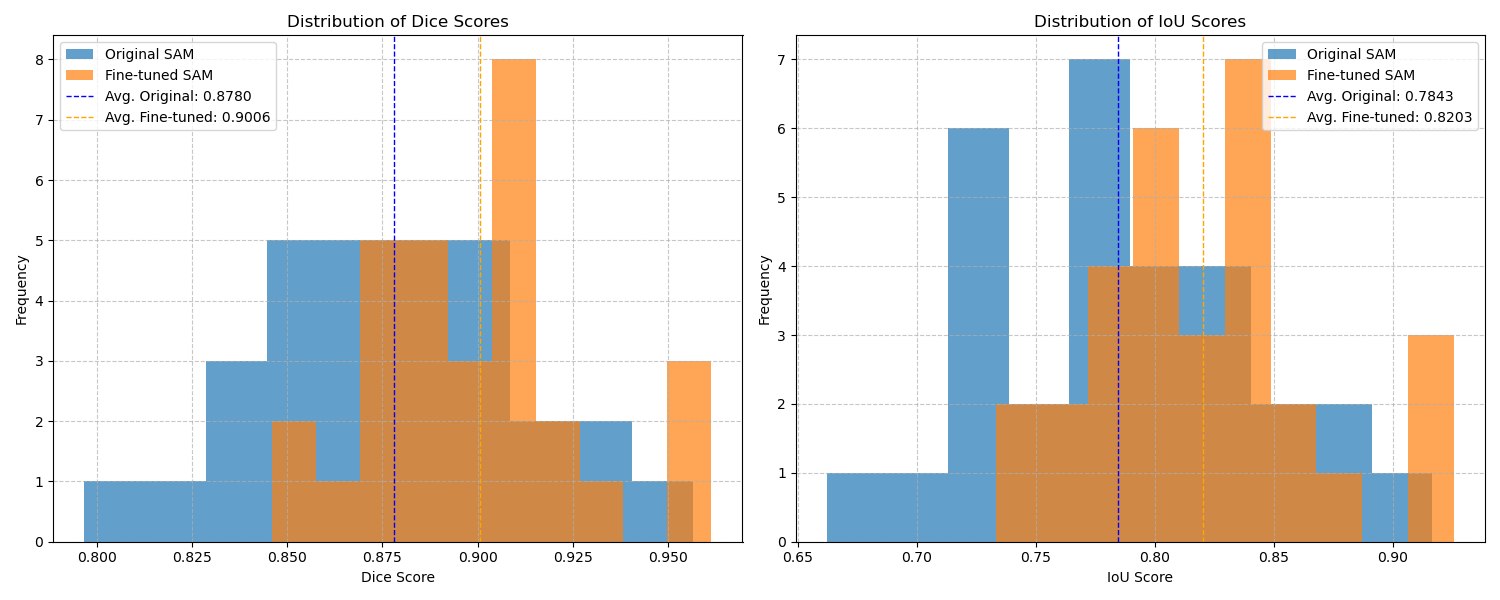
\includegraphics[width=\linewidth]{best_dice/best_dice_score_distributions.png}}}
  \caption{Best dice score distributions of SAM and CedarSAM, shifting towards the dotted line (indicating the average) to the right.}
  \label{fig:score_distributions}
\end{figure}

\begin{table}[h]
\centering
\caption{Best Dice Checkpoint: Dice and IoU Score Statistics}
\resizebox{\columnwidth}{!}{%
\begin{tabular}{|l||c|c|c|c|}
\hline
& \multicolumn{2}{c|}{\textbf{Dice Score}} & \multicolumn{2}{c|}{\textbf{IoU Score}} \\
\cline{2-5}
 & \textbf{SAM} & \textbf{CedarSAM} & \textbf{SAM} & \textbf{CedarSAM} \\
\hline
Minimum & 0.7968 & 0.8461 & 0.6622 & 0.7333 \\
\hline
Maximum & 0.9565 & 0.9613 & 0.9166 & 0.9255 \\
\hline
Mean & 0.8780 & 0.9006 & 0.7843 & 0.8203 \\
\hline
Q1 & 0.8503 & 0.8851 & 0.7395 & 0.7939 \\
\hline
Q3 & 0.9160 & 0.9255 & 0.8450 & 0.8614 \\
\hline
Std. Dev & 0.0412 & 0.0281 & 0.0632 & 0.0489 \\
\hline
\end{tabular}}
\label{tab:dice_iou_stats}
\end{table}

\section{Results and Discussion}
This section presents representative samples from the Best Dice, Best Loss, and Epoch 40 checkpoints to demonstrate the model's segmentation performance. Multiple examples are displayed for each checkpoint to provide a comprehensive comparison in visualization. For each sample, the results from both the original SAM and the fine-tuned model, CedarSAM are presented to illustrate the segmentation performance. The comparison uses a confusion matrix representation, highlighting different segmentation outcomes. True Positives (TP) are shown in green, representing correctly segmented regions where the model's predictions match the GT. False Positives (FP), displayed in blue, indicate areas incorrectly predicted as objects by the model when no actual object is present. False Negatives (FN) are highlighted in red, representing regions where the GT identifies an object, but the model fails to detect it.

\subsection{Dice Comparison}

The Dice score is used to evaluate the similarity between two sets of data, specifically the predicted segmentation mask and the annotated GT segmentation mask [18][19]. It ranges from 0, indicating no overlap, to 1, indicating a perfect match. This metric is particularly popular in medical image segmentation tasks because it is intuitive to understand and puts more emphasis on true positives while accounting for both FPs and FNs. Figures 5 and 6 illustrate the improvement from the original SAM model to CedarSAM, highlighting changes in FPs and FNs. In the top row, there are three images: The first one is original image, which is the actual UAV-captured image showing vegetation and other terrain. In the middle, it is a GT mask, which is the annotated mask representing vegetation regions in white in a binary format. The right one is original SAM prediction, displaying the output mask from the original SAM without training.

In the bottom row, there are three additional visualizations comparing the predictions with the GT mask. On the left, Original SAM vs GT presents the original SAM’s output with color-coded differences: Red indicates FNs, representing areas where vegetation was missed by SAM; Green shows TPs, representing correctly identified vegetation regions; and Blue marks FPs, representing areas incorrectly predicted as vegetation. In the middle, CedarSAM vs GT displays the same comparison for the CedarSAM, providing a clearer view of its improved segmentation performance. On the right, the visualization represents the results of the fine-tuning process applied to SAM, further illustrating its enhanced accuracy.

\begin{figure}[thpb]
  \centering
  \framebox{\parbox{3in}{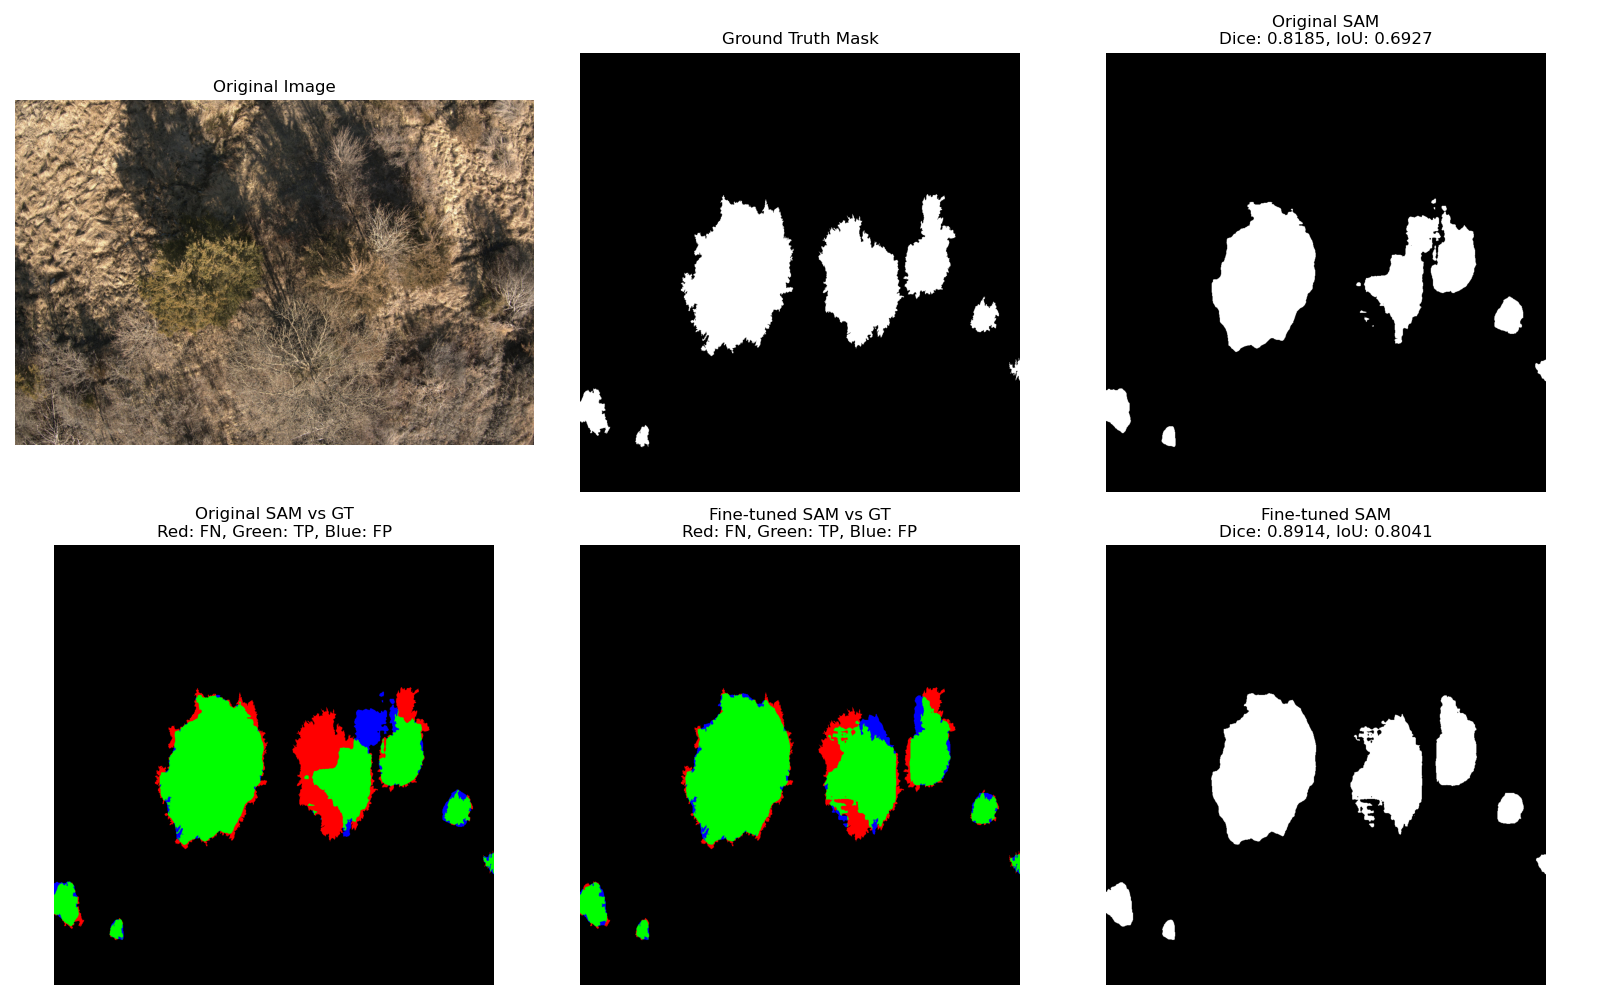
\includegraphics[width=\linewidth]{best_dice/sample_95_comparison.png}}}
  \caption{Sample 1: The original SAM scored a Dice of 0.82 and IoU of 0.69, while CedarSAM scored 0.89 and 0.8, respectively.}
  \label{fig:score_distributions}
\end{figure}

\begin{figure}[thpb]
  \centering
  \framebox{\parbox{3in}{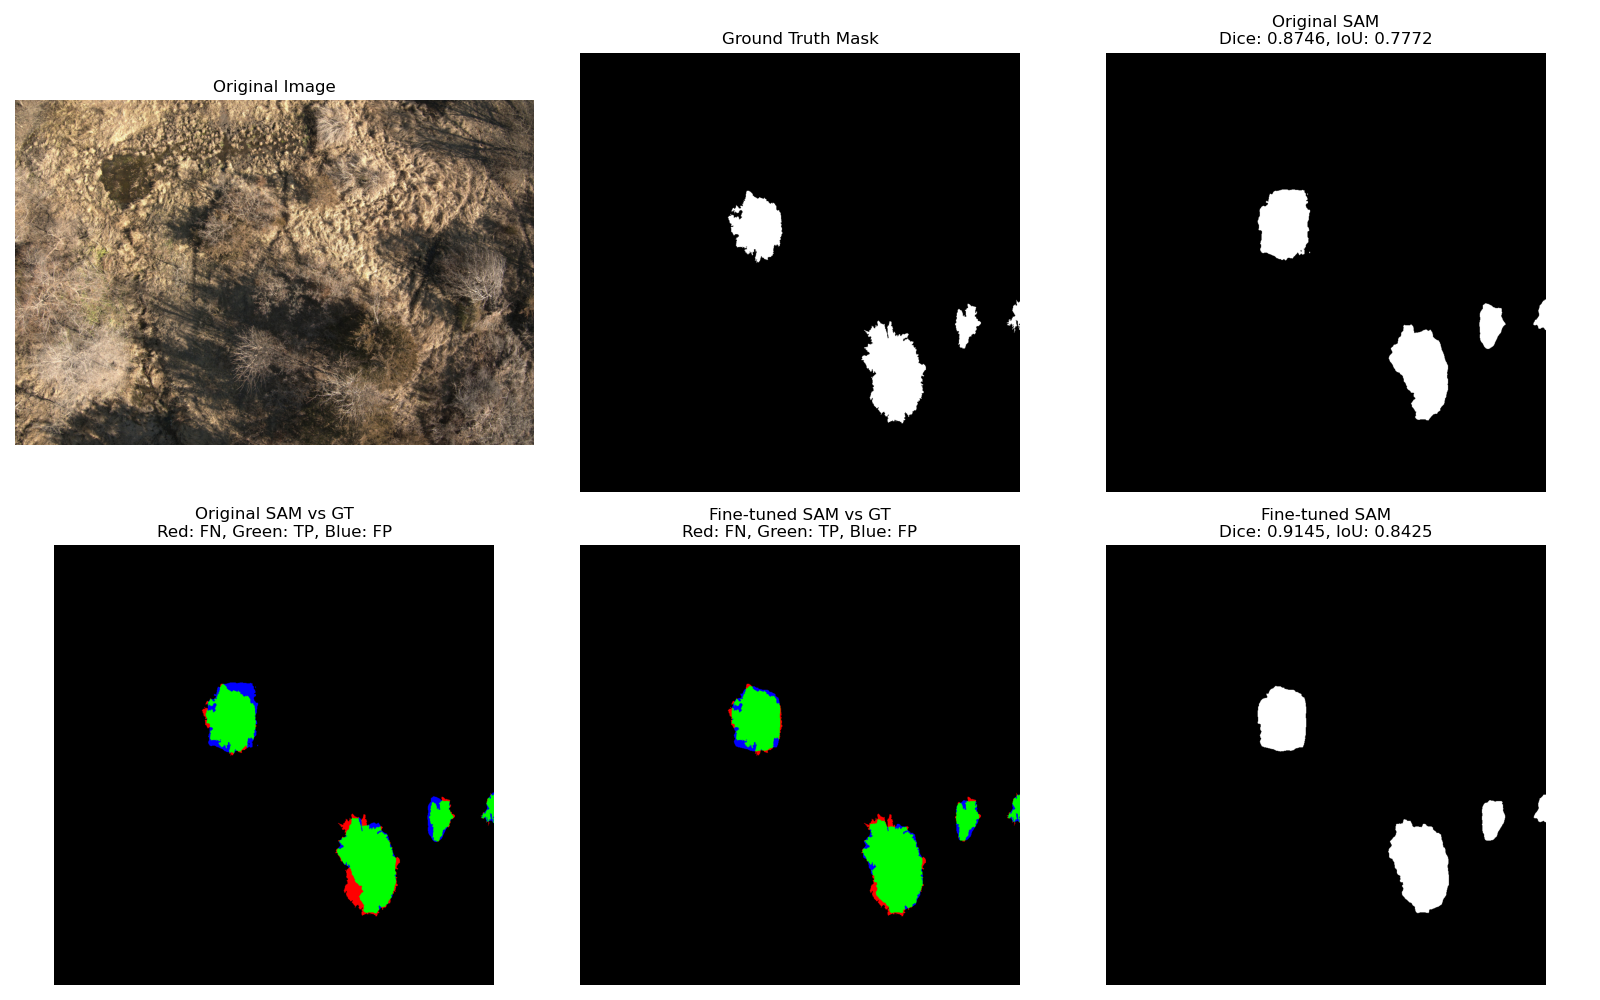
\includegraphics[width=\linewidth]{best_dice/sample_96_comparison.png}}}
  \caption{Sample 2: The original SAM scored a Dice of 0.87 and IoU of 0.78, whereas CedarSAM scored 0.91 and 0.84.}
  \label{fig:score_distributions}
\end{figure}

\subsection{Loss Comparison}
IoU tends to be more stringent than the Dice score because the denominator includes the entire union of both sets, meaning it penalizes errors more severely [20]. IoU calculates the ratio of the area of overlap (intersection) between the predicted segmentation and the GT to the area of their union. It ranges from 0, indicating no overlap, to 1, representing complete alignment. Figures 7 and 8 demonstrate the enhancement from the original SAM model to CedarSAM, emphasizing the differences in FPs and FNs.

\begin{figure}[thpb]
  \centering
  \framebox{\parbox{3in}{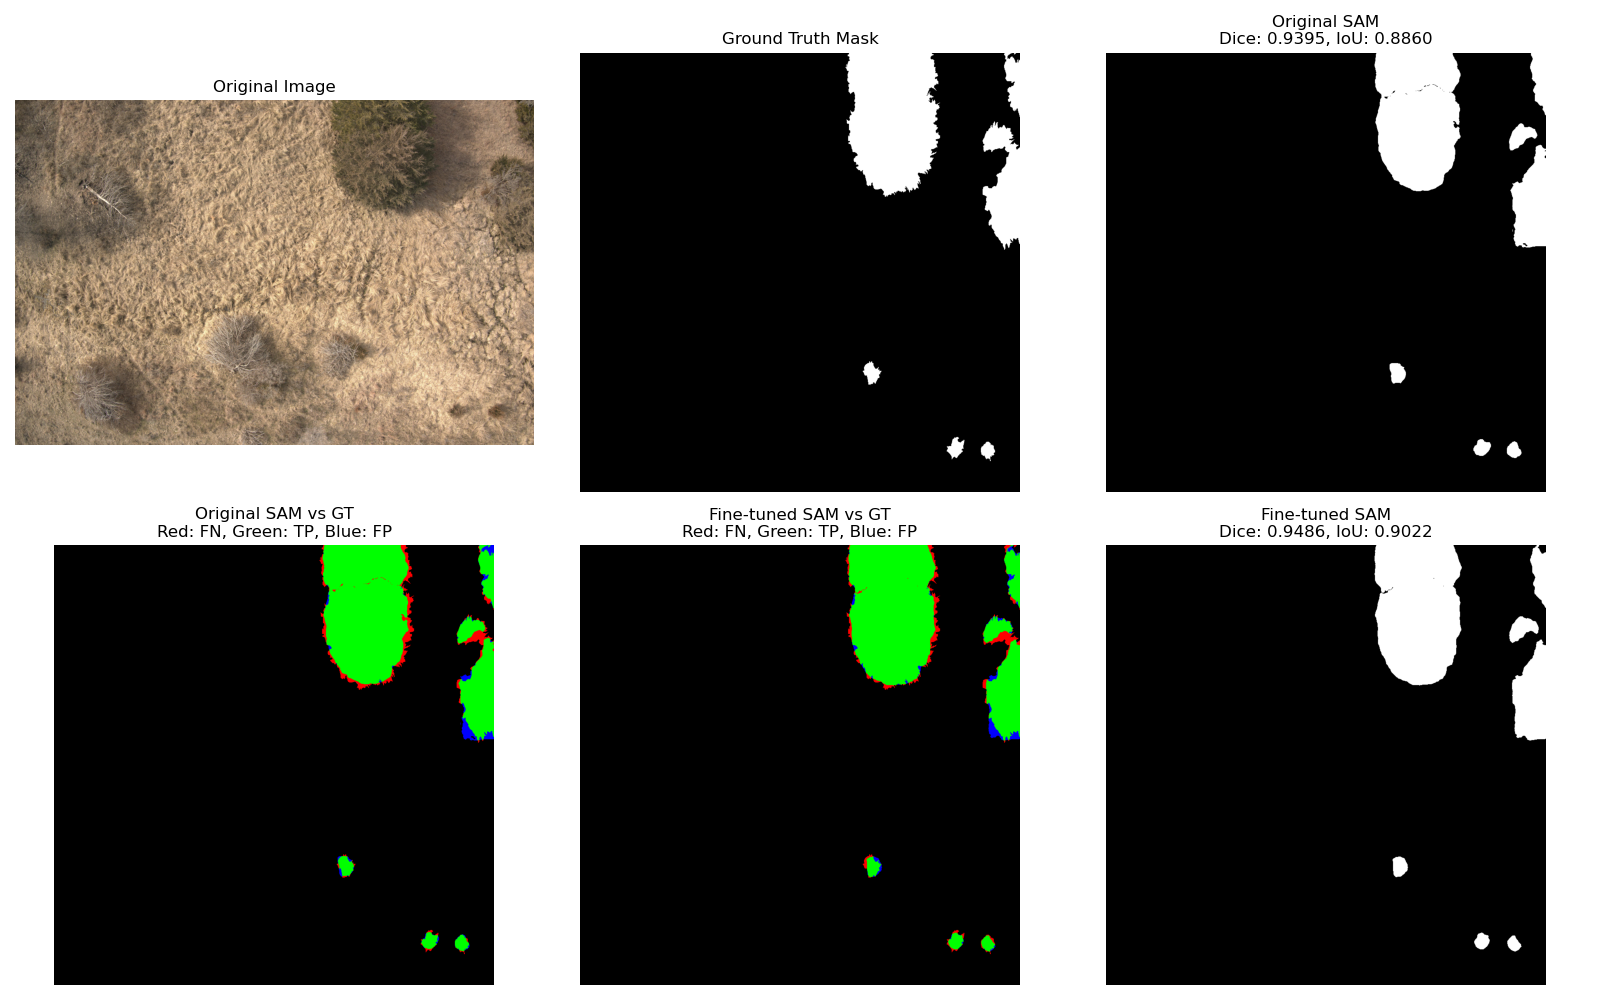
\includegraphics[width=\linewidth]{best_loss/sample_6_comparison.png}}}
  \caption{Sample 1: The original SAM shows segmentation performance with a 0.94 Dice score and 0.89 IoU score, while the CedarSAM variant demonstrated slightly enhanced results with a 0.95 Dice score and 0.90 IoU score following fine-tuning.}
  \label{fig:score_distributions}
\end{figure}

\begin{figure}[thpb]
  \centering
  \framebox{\parbox{3in}{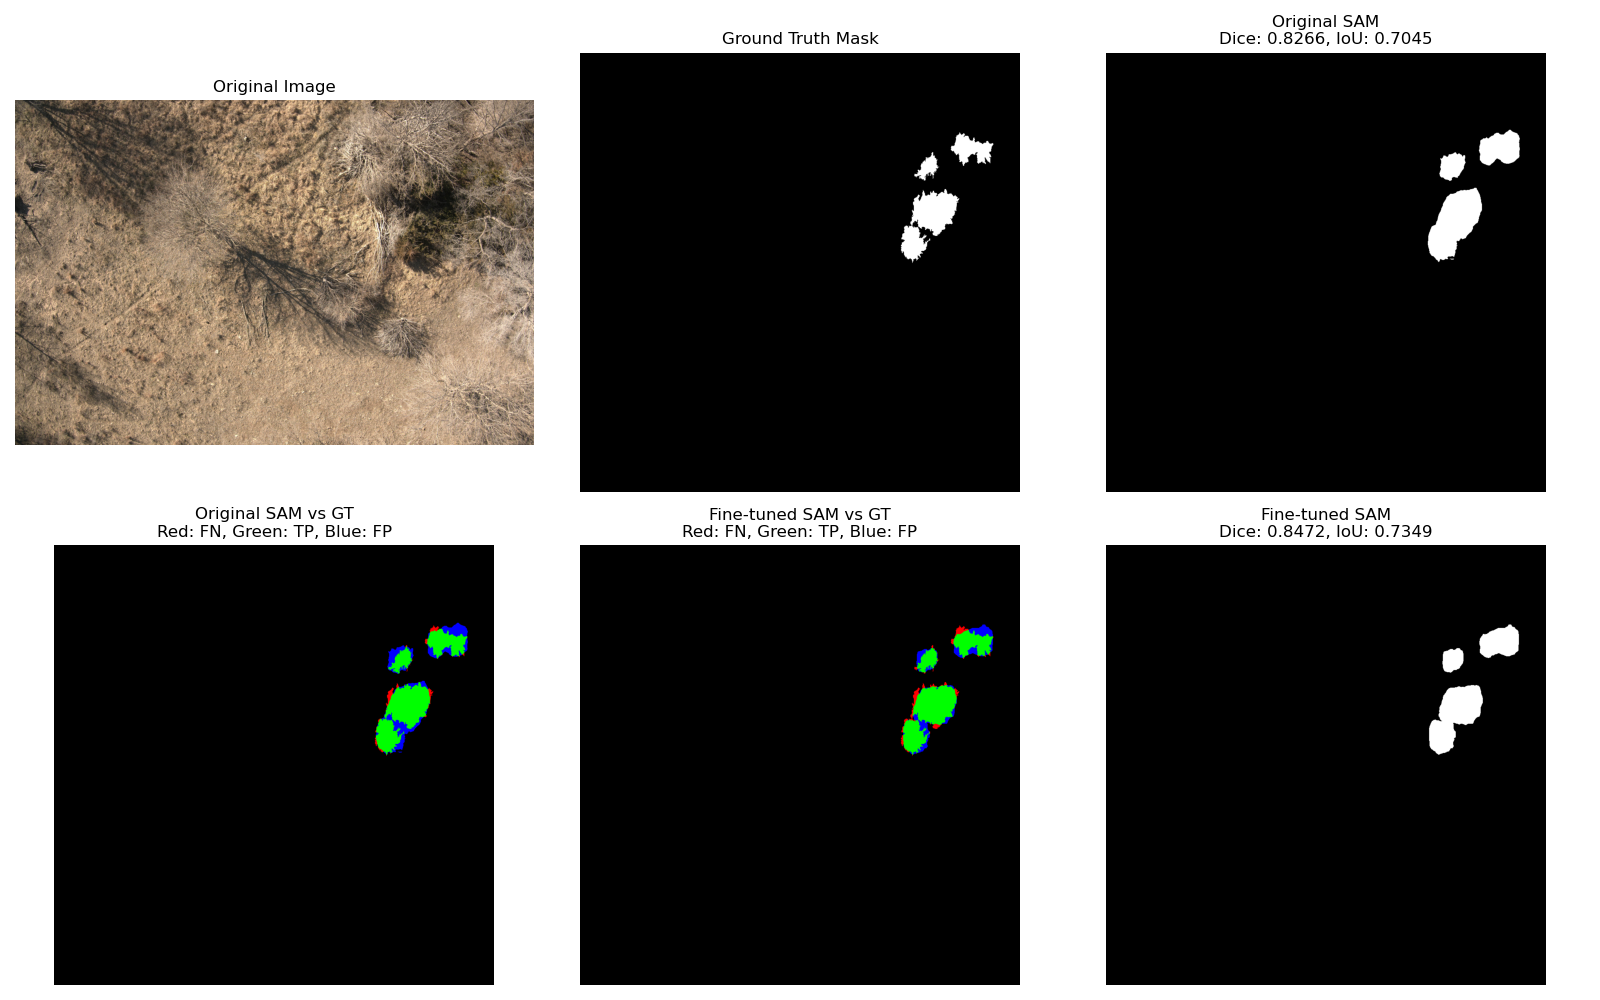
\includegraphics[width=\linewidth]{best_loss/sample_90_comparison.png}}}
  \caption{Sample 2: The original SAM achieved a Dice score of 0.83 and an IoU score of 0.70, while CedarSAM achieved a Dice score of 0.85 and an IoU score of 0.73.}
  \label{fig:score_distributions}
\end{figure}

\subsection{Number of Epoch Comparison}
An epoch refers to one complete pass of the entire training dataset through the neural network [21]. During each epoch, the model processes all training samples, adjusts its internal parameters (weights and biases), and aims to minimize the loss function [22]. Epoch 40 was selected as a representative since it showed the best results after completing multiple passes through the entire training dataset, as shown in Table 4. The table indicates that the highest Dice score was recorded at Epoch 40, achieving 0.9029 with a +1.96\% improvement. The best IoU was also observed at Epoch 40, reaching 0.8253 with a +3.50\% improvement. Additionally, the best Precision was recorded at Epoch 30 with a value of 0.9038 (+1.80\% improvement), while the highest Recall was achieved at Epoch 15, scoring 0.9209 (+3.45\% improvement).

\begin{table*}[h]
\centering
\caption{Performance Metrics by Epoch}
\resizebox{\textwidth}{!}{%
    \begin{tabular}{|c||c|c|c|c|c|c|c|c|}
        \hline
        \textbf{Epoch} & \textbf{Dice Score} & \textbf{IoU} & \textbf{Precision} & \textbf{Recall} & \textbf{Dice IMPR} & \textbf{IoU IMPR} & \textbf{Precision IMPR} & \textbf{Recall IMPR} \\
        \hline
        \textbf{Original} & 0.8855 & 0.7974 & 0.8878 & 0.8903 & -- & -- & -- & -- \\
        \hline
        5 & 0.8983 & 0.8179 & 0.8883 & 0.9119 & +0.0128 (+1.45\%) & +0.0206 (+2.58\%) & +0.0006 (+0.06\%) & +0.0217 (+2.44\%) \\
        \hline
        10 & 0.9006 & 0.8217 & 0.8947 & 0.9094 & +0.0151 (+1.71\%) & +0.0243 (+3.05\%) & +0.0069 (+0.78\%) & +0.0192 (+2.15\%) \\
        \hline
        15 & 0.8998 & 0.8207 & 0.8824 & 0.9209 & +0.0144 (+1.62\%) & +0.0233 (+2.92\%) & -0.0053 (-0.60\%) & +0.0307 (+3.45\%) \\
        \hline
        20 & 0.9004 & 0.8213 & 0.9009 & 0.9022 & +0.0150 (+1.69\%) & +0.0239 (+3.00\%) & +0.0131 (+1.48\%) & +0.0120 (+1.34\%) \\
        \hline
        25 & 0.9005 & 0.8216 & 0.8931 & 0.9103 & +0.0150 (+1.70\%) & +0.0242 (+3.04\%) & +0.0053 (+0.60\%) & +0.0200 (+2.25\%) \\
        \hline
        30 & 0.9018 & 0.8236 & 0.9038 & 0.9019 & +0.0163 (+1.85\%) & +0.0262 (+3.29\%) & +0.0160 (+1.80\%) & +0.0117 (+1.31\%) \\
        \hline
        35 & 0.9021 & 0.8241 & 0.9023 & 0.9038 & +0.0166 (+1.88\%) & +0.0267 (+3.35\%) & +0.0145 (+1.64\%) & +0.0135 (+1.52\%) \\
        \hline
        40 & 0.9029 & 0.8253 & 0.9026 & 0.9049 & +0.0174 (+1.96\%) & +0.0279 (+3.50\%) & +0.0149 (+1.68\%) & +0.0147 (+1.65\%) \\
        \hline
    \end{tabular}
}
\label{tab:performance}
\end{table*}

\begin{figure}[thpb]
  \centering
  \framebox{\parbox{3in}{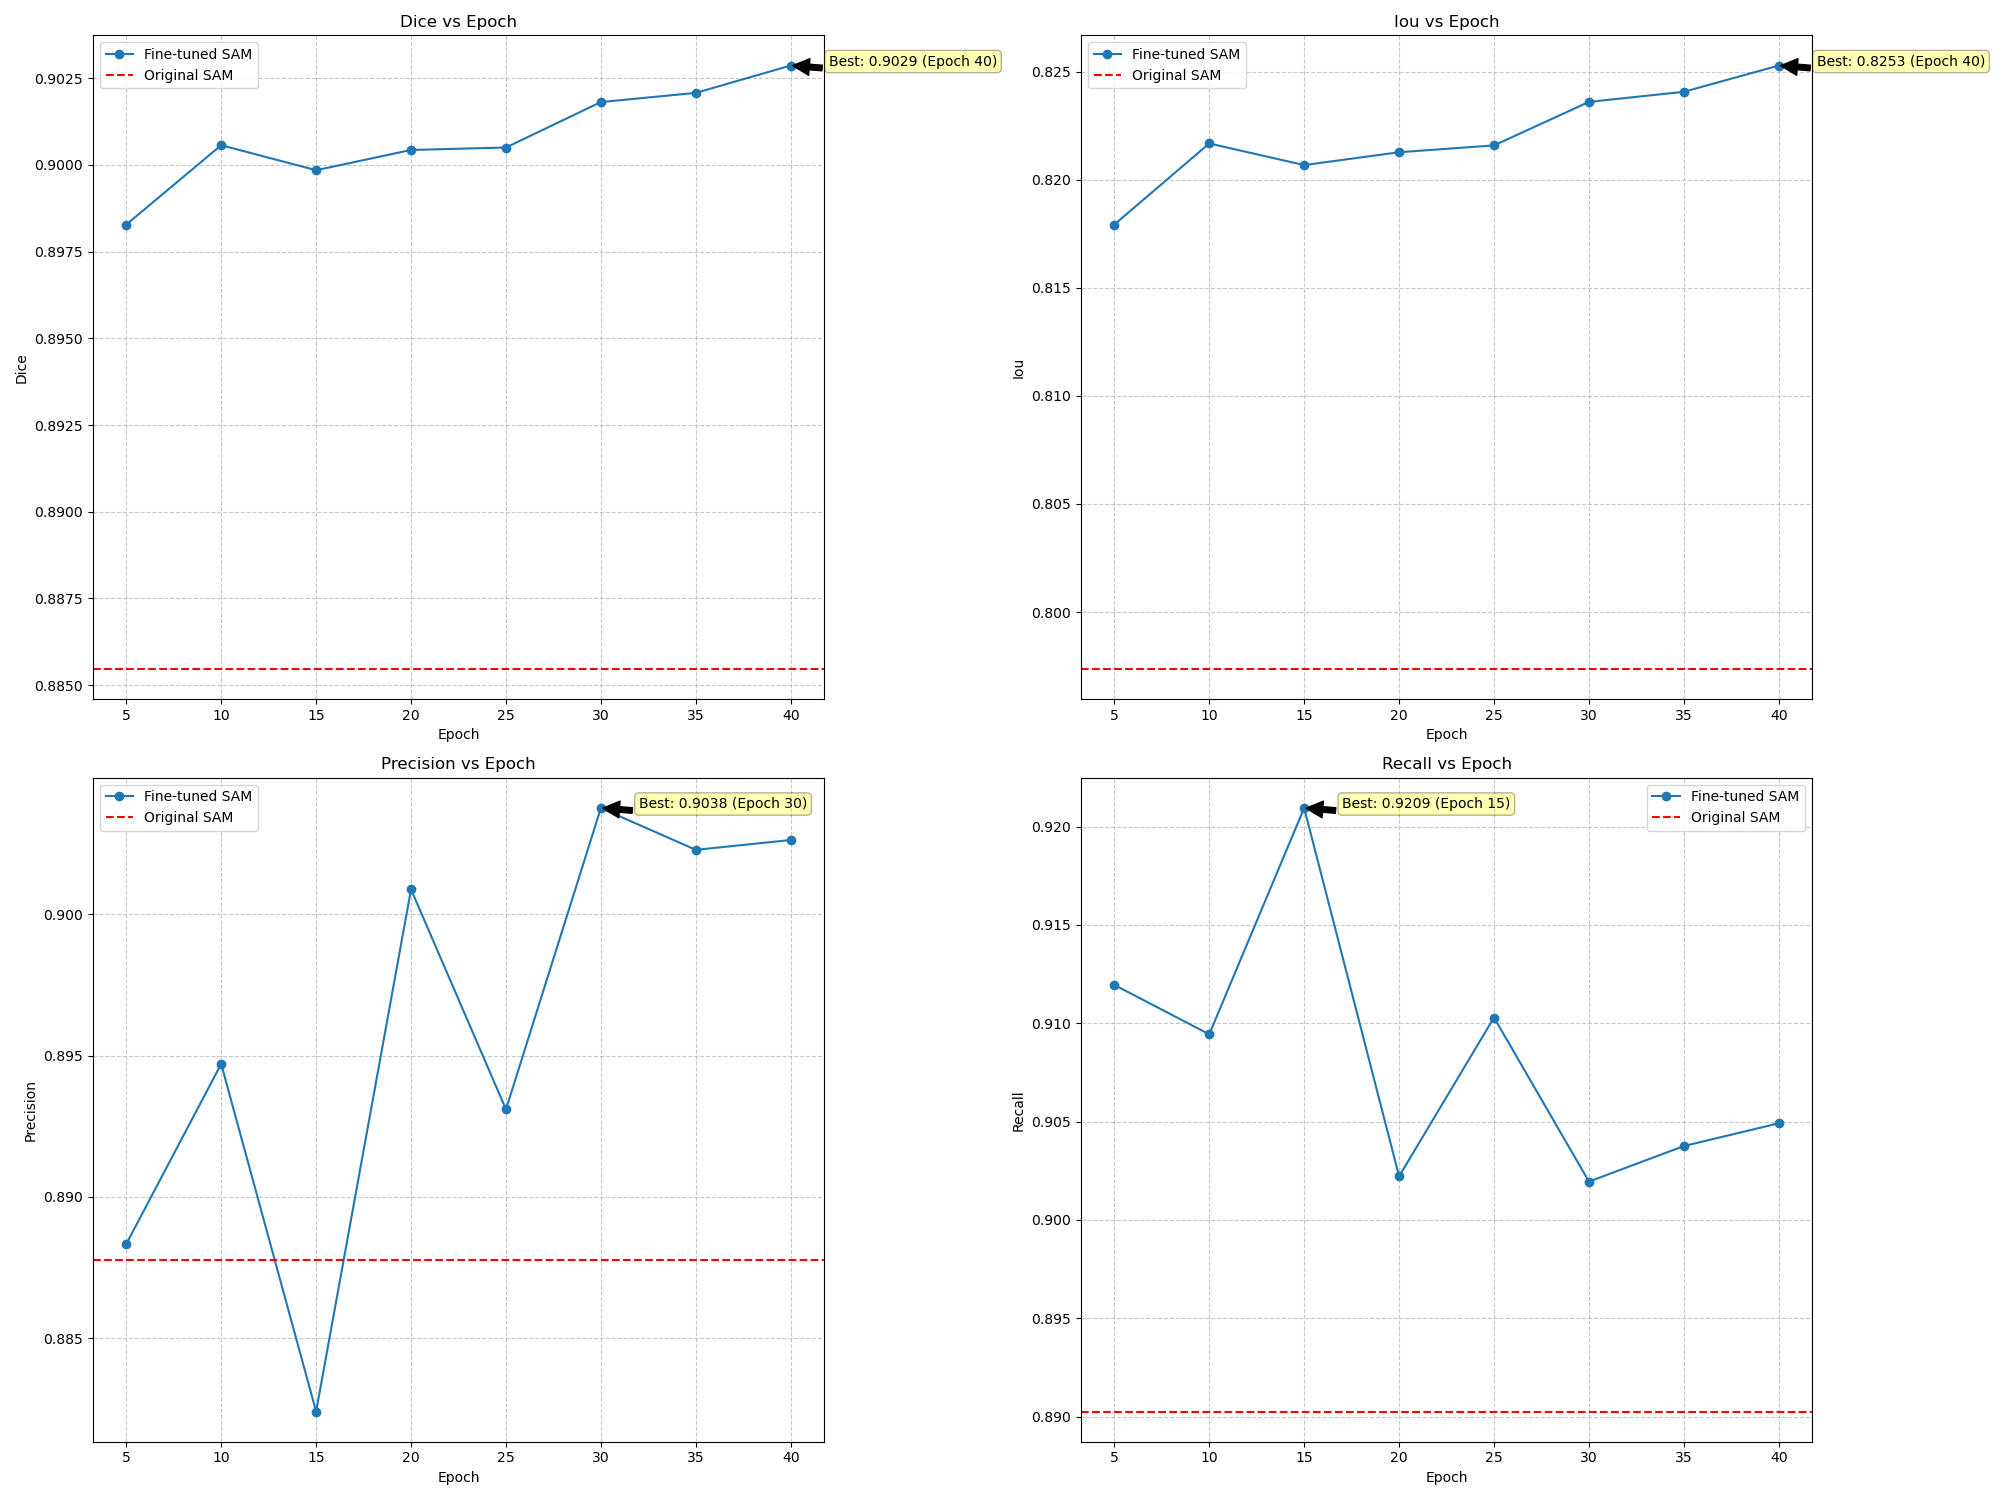
\includegraphics[width=\linewidth]{epoch40/metrics_across_epochs.png}}}
  \caption{Performance metrics of the CedarSAM across 40 epochs compared to the original SAM model.}
  \label{fig:score_distributions}
\end{figure}

Figure 9 illustrates the performance metrics of the CedarSAM across 40 epochs compared to the original SAM model. In the top left, the plot shows the Dice score. The fine-tuned CedarSAM model demonstrates a gradual improvement over epochs, reaching its highest Dice score of 0.9029 at Epoch 40. The red dashed line represents the original SAM's Dice score, which remains constant, indicating that the fine-tuned model consistently outperforms the original. The top right displays the IoU vs. Epoch. The fine-tuned SAM's IoU improves steadily, achieving its best IoU of 0.8253 at Epoch 40. The original SAM's IoU is again represented by a flat red dashed line, highlighting the substantial improvements gained through fine-tuning. In the bottom left, the plot shows Precision vs. Epoch. The fine-tuned SAM model experienced fluctuations in precision, peaking at 0.9038 at Epoch 30. The drop and recovery pattern suggests challenges in maintaining consistent precision during training, potentially due to factors such as class imbalance or varying segmentation difficulty. Finally, the bottom right plot shows Recall vs. Epoch. Recall peaked at 0.9209 at Epoch 15, indicating strong detection capability at that point. However, it declined in later epochs, which may suggest overfitting or reduced sensitivity to identifying vegetation regions. Given that most metrics plateau around Epoch 40, implementing early stopping at this point could be a suitable strategy to prevent overfitting while maintaining optimal performance.

\begin{figure}[thpb]
  \centering
  \framebox{\parbox{3in}{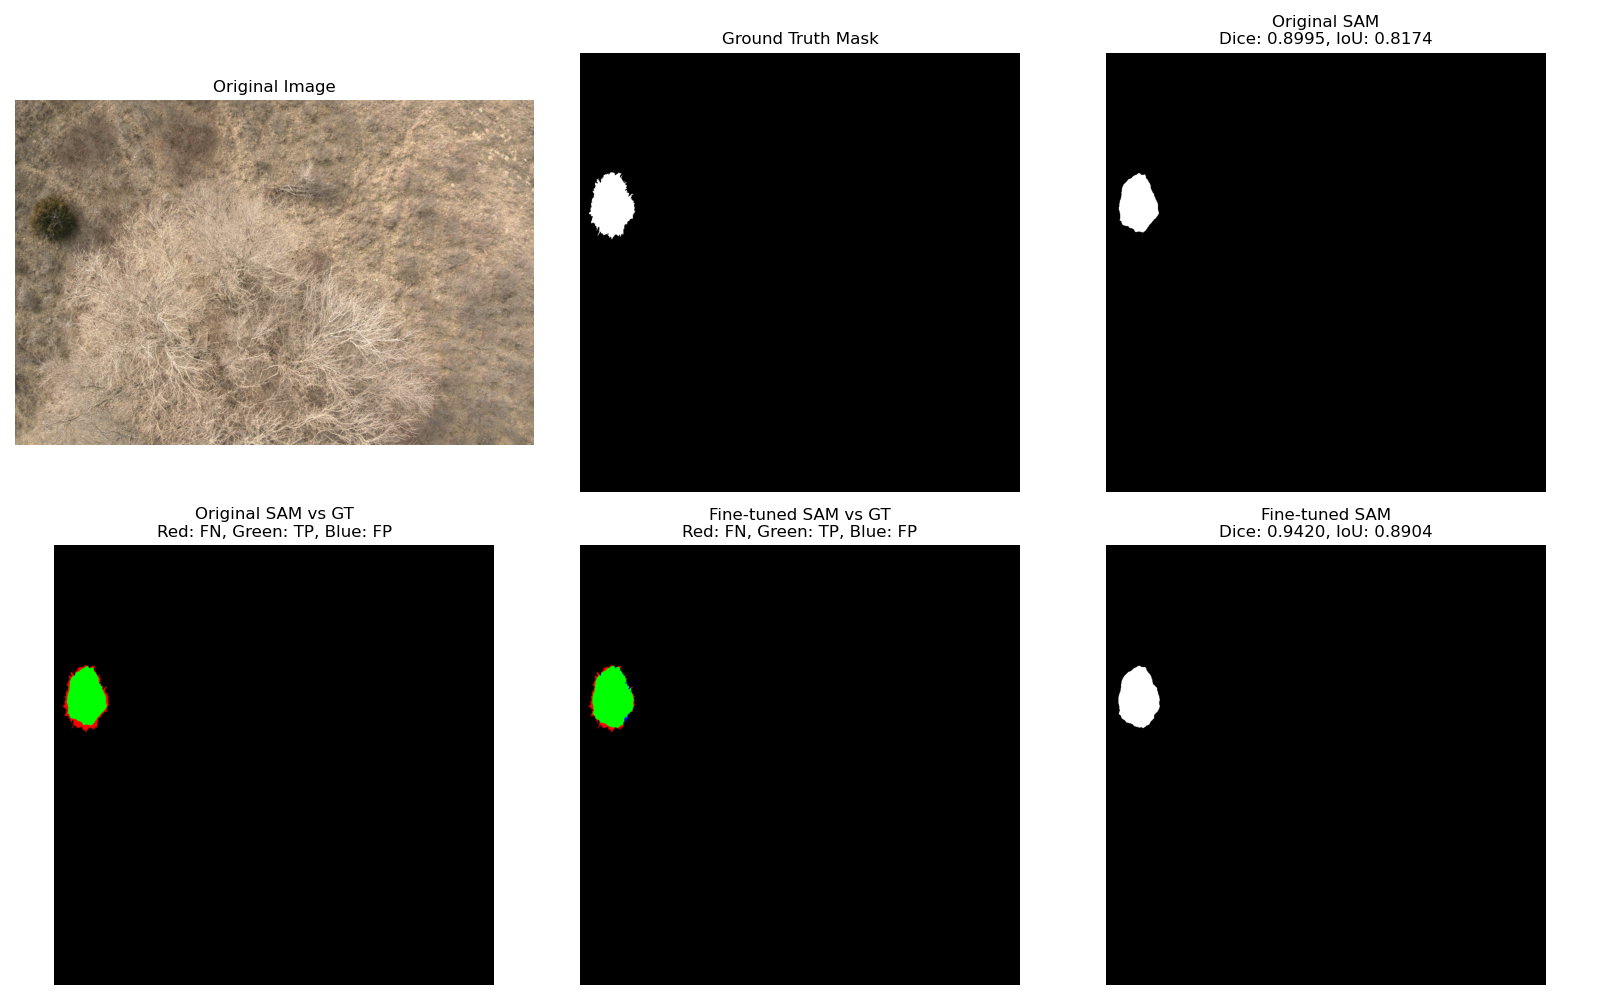
\includegraphics[width=\linewidth]{epoch40/sample_44_comparison.png}}}
  \caption{Sample 1: The original SAM achieved a Dice score of 0.90 and an IoU score of 0.82, while the fine-tuned CedarSAM achieved a Dice score of 0.94 and an IoU score of 0.89.}
  \label{fig:score_distributions}
\end{figure}

\begin{figure}[thpb]
  \centering
  \framebox{\parbox{3in}{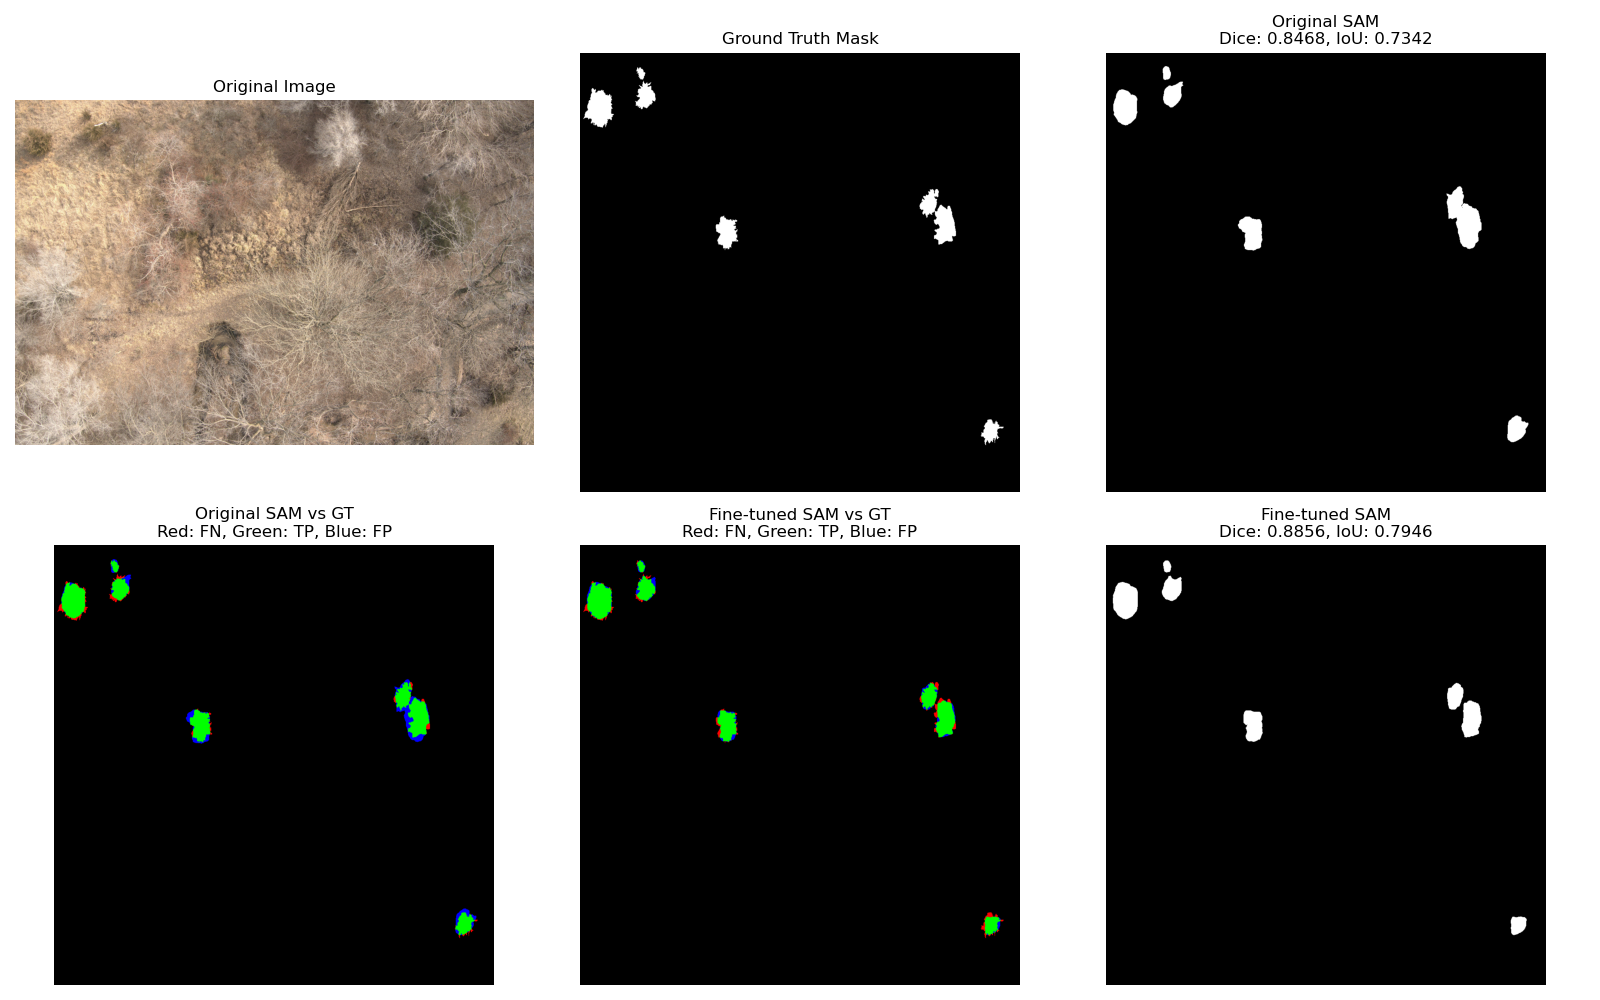
\includegraphics[width=\linewidth]{epoch40/sample_15_comparison.png}}}
  \caption{Sample 2: The original SAM achieved a Dice score of 0.85 and an IoU score of 0.73, while the fine-tuned CedarSAM achieved a Dice score of 0.89 and an IoU score of 0.79.}
  \label{fig:score_distributions}
\end{figure}

Lastly, Figures 10 and 11 provide examples comparing the Epoch 40 checkpoint of the CedarSAM with the original SAM. Both the single ERC tree and multiple tree scenarios demonstrate higher Dice and IoU scores, indicating improved segmentation accuracy.

\section{Results and Discussion}
The research demonstrates that the fine-tuned CedarSAM consistently outperforms the original SAM model in terms of segmentation accuracy and computational efficiency. CedarSAM achieved significant improvements across key evaluation metrics, including Dice score, IoU, Precision, and Recall. Moreover, inference time was reduced by up to 10.66\%, enhancing the model’s efficiency without sacrificing accuracy. These findings emphasize CedarSAM’s suitability for UAV-based ecological monitoring, where precise and efficient segmentation of vegetation is crucial. For example, CedarSAM reached a Dice score of 0.9029 (+1.96\%) and an IoU of 0.8253 (+3.50\%) at Epoch 40, indicating enhanced segmentation quality. While the Precision peaked at 0.9038 (+1.80\%) at Epoch 30, the highest Recall of 0.9209 (+3.45\%) was observed at Epoch 15. However, a slight decline in Recall at later epochs suggests potential overfitting, which could be mitigated using early stopping or adaptive learning rate strategies.

\section{CONCLUSIONS}
In this research, we aimed to demonstrate how a small dataset can effectively enhance the performance of a pretrained model through fine-tuning by addressing the following three questions: (1) How effectively can SAM be fine-tuned with a small domain-specific dataset? (2) What performance improvements can be expected across various evaluation metrics? (3) What are the trade-offs between model performance and computational efficiency after fine-tuning?

Despite the limited size of the dataset, the fine-tuned CedarSAM consistently outperformed the original SAM in terms of segmentation accuracy and computational efficiency. For future work, we plan to expand the dataset and conduct comparative studies to evaluate how dataset size impacts the model's performance. In addition, incorporating larger and more diverse datasets with images from different seasons, geographical regions, and environmental conditions will further enhance model robustness and mitigate overfitting. Improving the model's generalization capabilities will also be a key focus of future research. The findings of this study underscore the potential of adapting foundational models using small, high-quality datasets for specialized applications. This research contributes to the growing body of evidence that domain-specific fine-tuning can achieve robust performance without requiring extensive data collection, making it a practical and cost-effective solution for ecological monitoring.

\begin{thebibliography}{99}

\bibitem{c1} A. Kirillov, E. Mintun, N. Ravi, H. Mao, C. Rolland, L. Gustafson, and R. Girshick, ``Segment anything,'' in *Proc. IEEE/CVF Int. Conf. Comput. Vis.*, 2023.

\bibitem{c2} C. He, Y. Zhang, Q. Zhang, J. Yan, and X. Li, ``Weakly-supervised concealed object segmentation with SAM-based pseudo labeling and multi-scale feature grouping,'' *Adv. Neural Inf. Process. Syst.*, vol. 36, pp. 30726–30737, 2023.

\bibitem{c3} T. Chen, Y. Wang, Z. Li, X. Zhang, and J. Liu, ``SAM-Adapter: Adapting Segment Anything in underperformed scenes,'' in *Proc. IEEE/CVF Int. Conf. Comput. Vis.*, 2023.

\bibitem{c4} D.-P. Fan, G.-P. Ji, T. Zhou, G. Chen, H. Fu, and L. Shao, ``Concealed object detection,'' *IEEE Trans. Pattern Anal. Mach. Intell.*, vol. 44, no. 10, pp. 6024–6042, 2021.

\bibitem{c5} W. Ji, X. Zhang, Y. Li, H. Wang, and J. Zhao, ``Segment Anything is not always perfect: An investigation of SAM on different real-world applications,'' in *Proc. Conf.*, 2024, pp. 617–630.

\bibitem{c6} R. Kaur, O. Joshi, and R. E. Will, ``The ecological and economic determinants of eastern redcedar (Juniperus virginiana) encroachment in grassland and forested ecosystems: A case study from Oklahoma,'' *J. Environ. Manage.*, vol. 254, p. 109815, 2020.

\bibitem{c7} D. M. Meneguzzo and G. C. Liknes, ``Status and trends of eastern redcedar (Juniperus virginiana) in the central United States: Analyses and observations based on forest inventory and analysis data,'' *J. For.*, vol. 113, no. 3, pp. 325–334, 2015.

\bibitem{c8} A. M. Pierce and P. B. Reich, ``The effects of eastern red cedar (Juniperus virginiana) invasion and removal on a dry bluff prairie ecosystem,'' *Biol. Invasions*, vol. 12, pp. 241–252, 2010.

\bibitem{c9} Y. Diez, J. D. Wegner, K. Schindler, and J. A. Malo, ``Deep learning in forestry using UAV-acquired RGB data: A practical review,'' *Remote Sens.*, vol. 13, no. 14, p. 2837, 2021.

\bibitem{c10} M. Onishi and T. Ise, ``Explainable identification and mapping of trees using UAV RGB image and deep learning,'' *Sci. Rep.*, vol. 11, no. 1, p. 903, 2021.

\bibitem{c11} P. Bartmiński, M. Siłuch, and W. Kociuba, ``The effectiveness of a UAV-based LIDAR survey to develop digital terrain models and topographic texture analyses,'' *Sensors*, vol. 23, no. 14, p. 6415, 2023.

\bibitem{c12} S. Khan, M. Naseer, M. Hayat, S. W. Zamir, F. S. Khan, and M. Shah, ``Transformers in vision: A survey,'' *ACM Comput. Surv. (CSUR)*, vol. 54, no. 10s, pp. 1–41, 2022.

\bibitem{c13} H. Chang, H. Qi, S. Gidaris, J. Zhang, L. Sigal, and D. Cai, ``MaskGIT: Masked generative image transformer,'' in *Proc. IEEE/CVF Conf. Comput. Vis. Pattern Recognit.*, 2022.

\bibitem{c14} M. M. Taye, ``Theoretical understanding of convolutional neural network: Concepts, architectures, applications, future directions,'' *Computation*, vol. 11, no. 3, p. 52, 2023.

\bibitem{c15} C. Zhang, Y. Wang, Z. Li, X. Zhang, and J. Liu, ``A comprehensive survey on Segment Anything Model for vision and beyond,'' *arXiv preprint arXiv:2305.08196*, 2023.

\bibitem{c16} W. Xie, Y. Zhang, J. Liu, and H. Li, ``SAM fewshot finetuning for anatomical segmentation in medical images,'' in *Proc. IEEE/CVF Winter Conf. Appl. Comput. Vis.*, 2024.

\bibitem{c17} L. Ke, M. Wu, X. Zhang, Z. Liu, and S. Lin, ``Segment anything in high quality,'' *Adv. Neural Inf. Process. Syst.*, vol. 36, pp. 29914–29934, 2023.

\bibitem{c18} D. Müller, I. Soto-Rey, and F. Kramer, ``Towards a guideline for evaluation metrics in medical image segmentation,'' *BMC Res. Notes*, vol. 15, no. 1, p. 210, 2022.

\bibitem{c19} F. Kofler, M. Muehlburger, D. Ritt, J. Gomez, and J. Pfeuffer, ``Are we using appropriate segmentation metrics? Identifying correlates of human expert perception for CNN training beyond rolling the DICE coefficient,'' *arXiv preprint arXiv:2103.06205*, 2021.

\bibitem{c20} Y.-J. Cho, ``Weighted Intersection over Union (wIoU) for evaluating image segmentation,'' *arXiv preprint arXiv:2107.09858*, 2021.

\bibitem{c21} M. Sun, H. Zhang, L. Fan, and H. Su, ``Understanding architecture age and style through deep learning,'' *Cities*, vol. 128, p. 103787, 2022.

\bibitem{c22} M. Li, Y. Sun, X. Liu, and J. Zhao, ``Autobalance: Optimized loss functions for imbalanced data,'' *Adv. Neural Inf. Process. Syst.*, vol. 34, pp. 3163–3177, 2021.

\end{thebibliography}
\end{document}
